\documentclass[border=16pt, tikz]{standalone}
\usepackage[T1]{fontenc}
\usepackage{helvet}
\renewcommand{\familydefault}{\sfdefault}
\usepackage{amsmath, amssymb}
\usetikzlibrary{arrows.meta, positioning, calc, backgrounds, fit}

% Color Palette (Matching V4 Figures)
\definecolor{slateDark}{HTML}{0F172A}
\definecolor{slateText}{HTML}{334155}
\definecolor{slateMuted}{HTML}{64748B}
\definecolor{slateBorder}{HTML}{CBD5E1}
\definecolor{slateBg}{HTML}{F8FAFC}

\definecolor{redDark}{HTML}{991B1B}
\definecolor{redBorder}{HTML}{EF4444}
\definecolor{redBg}{HTML}{FEF2F2}

\definecolor{blueDark}{HTML}{0369A1}
\definecolor{blueMain}{HTML}{0284C7}
\definecolor{blueBg}{HTML}{F0F9FF}

\definecolor{purpleDark}{HTML}{5B21B6}
\definecolor{purpleMain}{HTML}{7C3AED}
\definecolor{purpleBg}{HTML}{F5F3FF}

\definecolor{greenDark}{HTML}{047857}
\definecolor{greenMain}{HTML}{059669}
\definecolor{greenBg}{HTML}{ECFDF5}

\definecolor{amberDark}{HTML}{B45309}
\definecolor{amberMain}{HTML}{D97706}
\definecolor{amberBg}{HTML}{FFFBEB}

\begin{document}
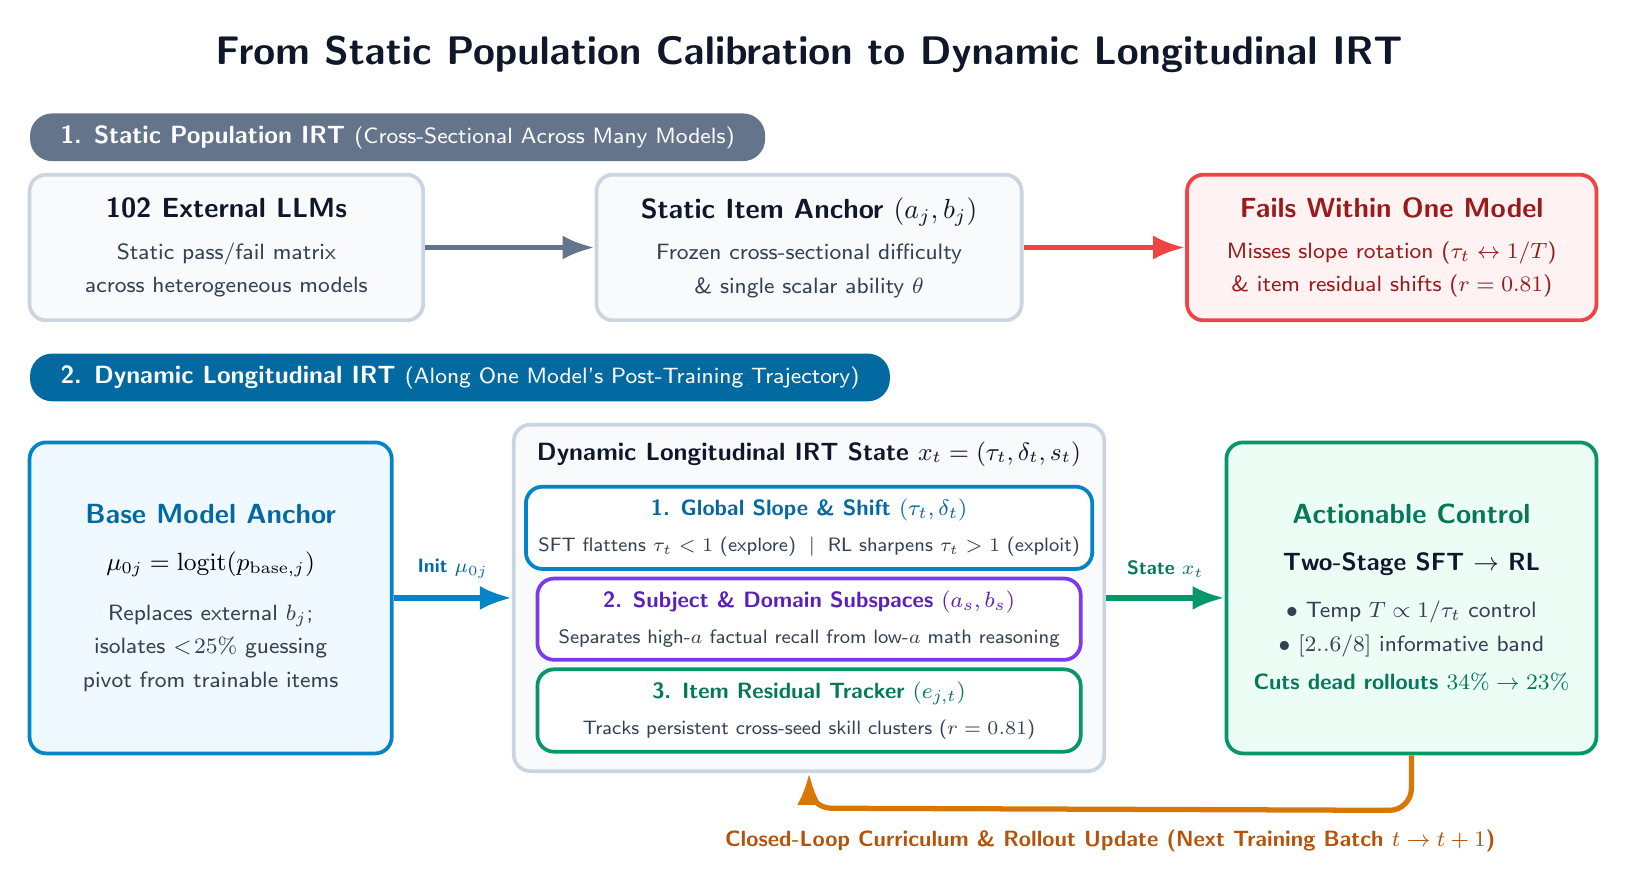
\begin{tikzpicture}[
    >=Latex,
    font=\sffamily,
    box/.style={
        rectangle,
        rounded corners=6pt,
        draw=#1,
        line width=1.35pt,
        fill=white,
        align=center,
        inner sep=8pt
    },
    pill/.style={
        rectangle,
        rounded corners=8pt,
        fill=#1,
        text=white,
        font=\sffamily\bfseries\small,
        inner xsep=11pt,
        inner ysep=4.5pt
    },
    arrow/.style={
        ->,
        line width=1.9pt,
        color=#1
    }
]

% ============================================================================
% TITLE
% ============================================================================
\node[font=\sffamily\bfseries\Large, text=slateDark] (title) at (0, 7.25)
    {From Static Population Calibration to Dynamic Longitudinal IRT};

% ============================================================================
% ROW 1: STATIC POPULATION IRT (TOP)
% ============================================================================
\node[pill=slateMuted, anchor=west] (p1) at (-9.9, 6.2)
    {1. Static Population IRT \normalfont\footnotesize (Cross-Sectional Across Many Models)};

\node[box=slateBorder, fill=slateBg, minimum width=5.0cm, minimum height=1.85cm] (s1) at (-7.4, 4.8) {
    \textbf{\color{slateDark} 102 External LLMs}\\[3pt]
    {\footnotesize\color{slateText} Static pass/fail matrix}\\
    {\footnotesize\color{slateText} across heterogeneous models}
};

\node[box=slateBorder, fill=slateBg, minimum width=5.4cm, minimum height=1.85cm] (s2) at (0.0, 4.8) {
    \textbf{\color{slateDark} Static Item Anchor $(a_j, b_j)$}\\[3pt]
    {\footnotesize\color{slateText} Frozen cross-sectional difficulty}\\
    {\footnotesize\color{slateText} \& single scalar ability $\theta$}
};

\node[box=redBorder, fill=redBg, minimum width=5.2cm, minimum height=1.85cm] (s3) at (7.4, 4.8) {
    \textbf{\color{redDark} Fails Within One Model}\\[3pt]
    {\footnotesize\color{redDark} Misses slope rotation ($\tau_t \leftrightarrow 1/T$)}\\
    {\footnotesize\color{redDark} \& item residual shifts ($r = 0.81$)}
};

\draw[arrow=slateMuted] (s1.east) -- (s2.west);
\draw[arrow=redBorder]  (s2.east) -- (s3.west);

% ============================================================================
% ROW 2: DYNAMIC LONGITUDINAL IRT (BOTTOM CLOSED LOOP)
% ============================================================================
\node[pill=blueDark, anchor=west] (p2) at (-9.9, 3.15)
    {2. Dynamic Longitudinal IRT \normalfont\footnotesize (Along One Model's Post-Training Trajectory)};

% Left Node: Base Coordinate Anchor
\node[box=blueMain, fill=blueBg, minimum width=4.6cm, minimum height=3.95cm] (d1) at (-7.6, 0.35) {
    \textbf{\color{blueDark} Base Model Anchor}\\[5pt]
    {\small $\mu_{0j} = \mathrm{logit}(p_{\mathrm{base},j})$}\\[6pt]
    {\footnotesize\color{slateText} Replaces external $b_j$;}\\
    {\footnotesize\color{slateText} isolates $<\!25\%$ guessing}\\
    {\footnotesize\color{slateText} pivot from trainable items}
};

% Center Engine Box (3 Stacked Layers)
\node[box=slateBorder, fill=slateBg, minimum width=7.5cm, minimum height=4.4cm] (engine_bg) at (0.0, 0.35) {};
\node[font=\sffamily\bfseries\small, text=slateDark] at (0.0, 2.18)
    {Dynamic Longitudinal IRT State $x_t = (\tau_t, \delta_t, s_t)$};

\node[box=blueMain, fill=white, minimum width=6.9cm, minimum height=0.95cm, inner sep=4.5pt] (e1) at (0.0, 1.24) {
    \textbf{\footnotesize\color{blueDark} 1. Global Slope \& Shift $(\tau_t, \delta_t)$}\\[1pt]
    {\scriptsize\color{slateText} SFT flattens $\tau_t < 1$ (explore) \;\textbar\; RL sharpens $\tau_t > 1$ (exploit)}
};

\node[box=purpleMain, fill=white, minimum width=6.9cm, minimum height=0.95cm, inner sep=4.5pt] (e2) at (0.0, 0.08) {
    \textbf{\footnotesize\color{purpleDark} 2. Subject \& Domain Subspaces $(a_s, b_s)$}\\[1pt]
    {\scriptsize\color{slateText} Separates high-$a$ factual recall from low-$a$ math reasoning}
};

\node[box=greenMain, fill=white, minimum width=6.9cm, minimum height=0.95cm, inner sep=4.5pt] (e3) at (0.0, -1.08) {
    \textbf{\footnotesize\color{greenDark} 3. Item Residual Tracker $(e_{j,t})$}\\[1pt]
    {\scriptsize\color{slateText} Tracks persistent cross-seed skill clusters ($r = 0.81$)}
};

% Right Node: Actionable Training Control
\node[box=greenMain, fill=greenBg, minimum width=4.7cm, minimum height=3.95cm] (d3) at (7.65, 0.35) {
    \textbf{\color{greenDark} Actionable Control}\\[5pt]
    {\small\color{slateDark} \textbf{Two-Stage SFT $\rightarrow$ RL}}\\[5pt]
    {\footnotesize\color{slateText} $\bullet$ Temp $T \propto 1/\tau_t$ control}\\
    {\footnotesize\color{slateText} $\bullet$ $[2..6/8]$ informative band}\\[2pt]
    {\footnotesize\color{greenDark} \textbf{Cuts dead rollouts $34\% \rightarrow 23\%$}}
};

% Forward Arrows
\draw[arrow=blueMain] (d1.east) -- node[above=3pt, font=\sffamily\bfseries\scriptsize, text=blueDark] {Init $\mu_{0j}$} (engine_bg.west);
\draw[arrow=greenMain] (engine_bg.east) -- node[above=3pt, font=\sffamily\bfseries\scriptsize, text=greenDark] {State $x_t$} (d3.west);

% Bottom Closed-Loop Feedback Arrow
\draw[arrow=amberMain, rounded corners=8pt]
    (d3.south) -- ++(0, -0.70)
    -- node[below=3pt, font=\sffamily\bfseries\footnotesize, text=amberDark]
       {Closed-Loop Curriculum \& Rollout Update (Next Training Batch $t \rightarrow t+1$)}
       (0.0, -2.32)
    -| (engine_bg.south);

\end{tikzpicture}
\end{document}
